\subsection{Wirelessmodul}
\label{subsec:Wirelessmodul}

Über einen Web-Host soll der User die Möglickeit haben, Getränke auszuwähen und seinem RFID-Chip zuzuordnen, sowie diverse kleinere Einstellungen an der Maschine vorzunemen. Dazu wird ein WiFi-Modul benötigt.

Aufgrund schon bestehender Erfahrungen wurde ein Espressif ESP-Modul ausgewählt. Grundsätzlich standen zwei Modelle zur Auswahl. Das ESP8266 und das ESP32. Für die Cocktailmaschine wurde das ESP32 ausgewählt, da dies einfach Leistungsstärker ist. Die genauen Datenvergleiche sind in Tabelle \ref{tab:ESP} ersichtlich.

\begin{table}[!h]
\begin{tabularx}{\textwidth}{l|X|X}
MCU                    & Xtensa Single-core 32-bit L106 & Xtensa Dual-Core 32-bit LX6 \\ \hline
802.11 b/g/n     		& HT20                           & HT40                                       \\
Bluetooth              	& No                             & Bluetooth 4.2 and BLE                      \\
Arbeitsfrequenz			& 80 MHz                         & 160 MHz                                    \\
SRAM                   	& No                             & Yes                                         \\
Flash                  	& No                             & Yes                                          \\
GPIO                   	& 17                             & 36                                         \\
SPI/I2C/I2S/UART       	& 2/1/2/2                        & 4/2/2/2                                    \\
ADC                    	& 10-bit                         & 12-bit                                     \\
Ethernet Interface 		& No                             & Yes                                          \\
Touchsensor           	& No                             & Yes                                          \\
Temperatursensor     	& No                             & Yes                                          \\
Hall-Sensor     		& No                             & Yes \\
Arbeitstemperatur    	& -40ºC to 125ºC                 & -40ºC to 125ºC                             \\
Price                  	& \$ (3\$ - \$6)                   & \$\$ (\$6 - \$12)                             
\end{tabularx}
\caption{Vergleich ESP8266 zu ESP32.}
\label{tab:ESP}
\end{table}

Wichtig ist, dass ein ESP ausgewählt wird, welches einen Anschluss für eine abgesetzte Antenne hat, da die Leiterplatte, worauf das Modul verbaut wird, im Gehäuse platziert wird. Dazu eignet sich der Espressif ESP32-32U. Dieses ist in Abbildung \ref{fig:Produktbild_ESP32_32U_Wroom} als Wroom dargestellt und in Abbildung \ref{fig:Produktbild_ESP32_32U_DevKit} als Development Kit.

Das ESP32 unterstützt das Protokoll nach ISO 802.11 b/g/n und kann somit auf 2.4GHz sowie 5GHz arbeiten. Mit dem n-Protokoll und einer Antenne kann so bis zu 150MBit übertragen werden bei einer Bandbreite von 20MHz.

\begin{figure}[!h]
\center
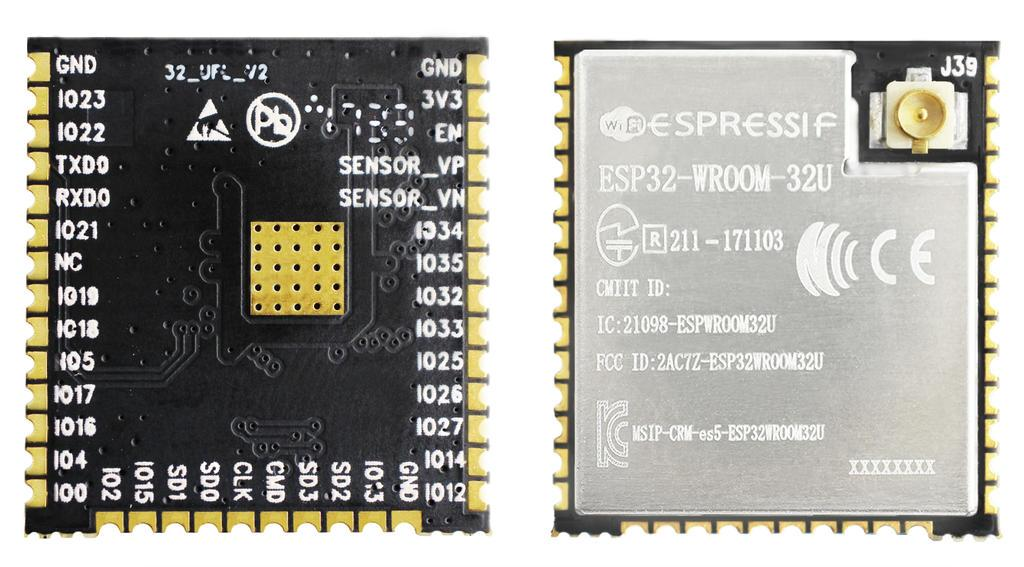
\includegraphics[width = 0.4\textwidth]{graphics/Produktbild_ESP32}
\caption{ESP32-32U Wroom.}
\label{fig:Produktbild_ESP32_32U_Wroom}
\end{figure}

\begin{figure}[!h]
\center
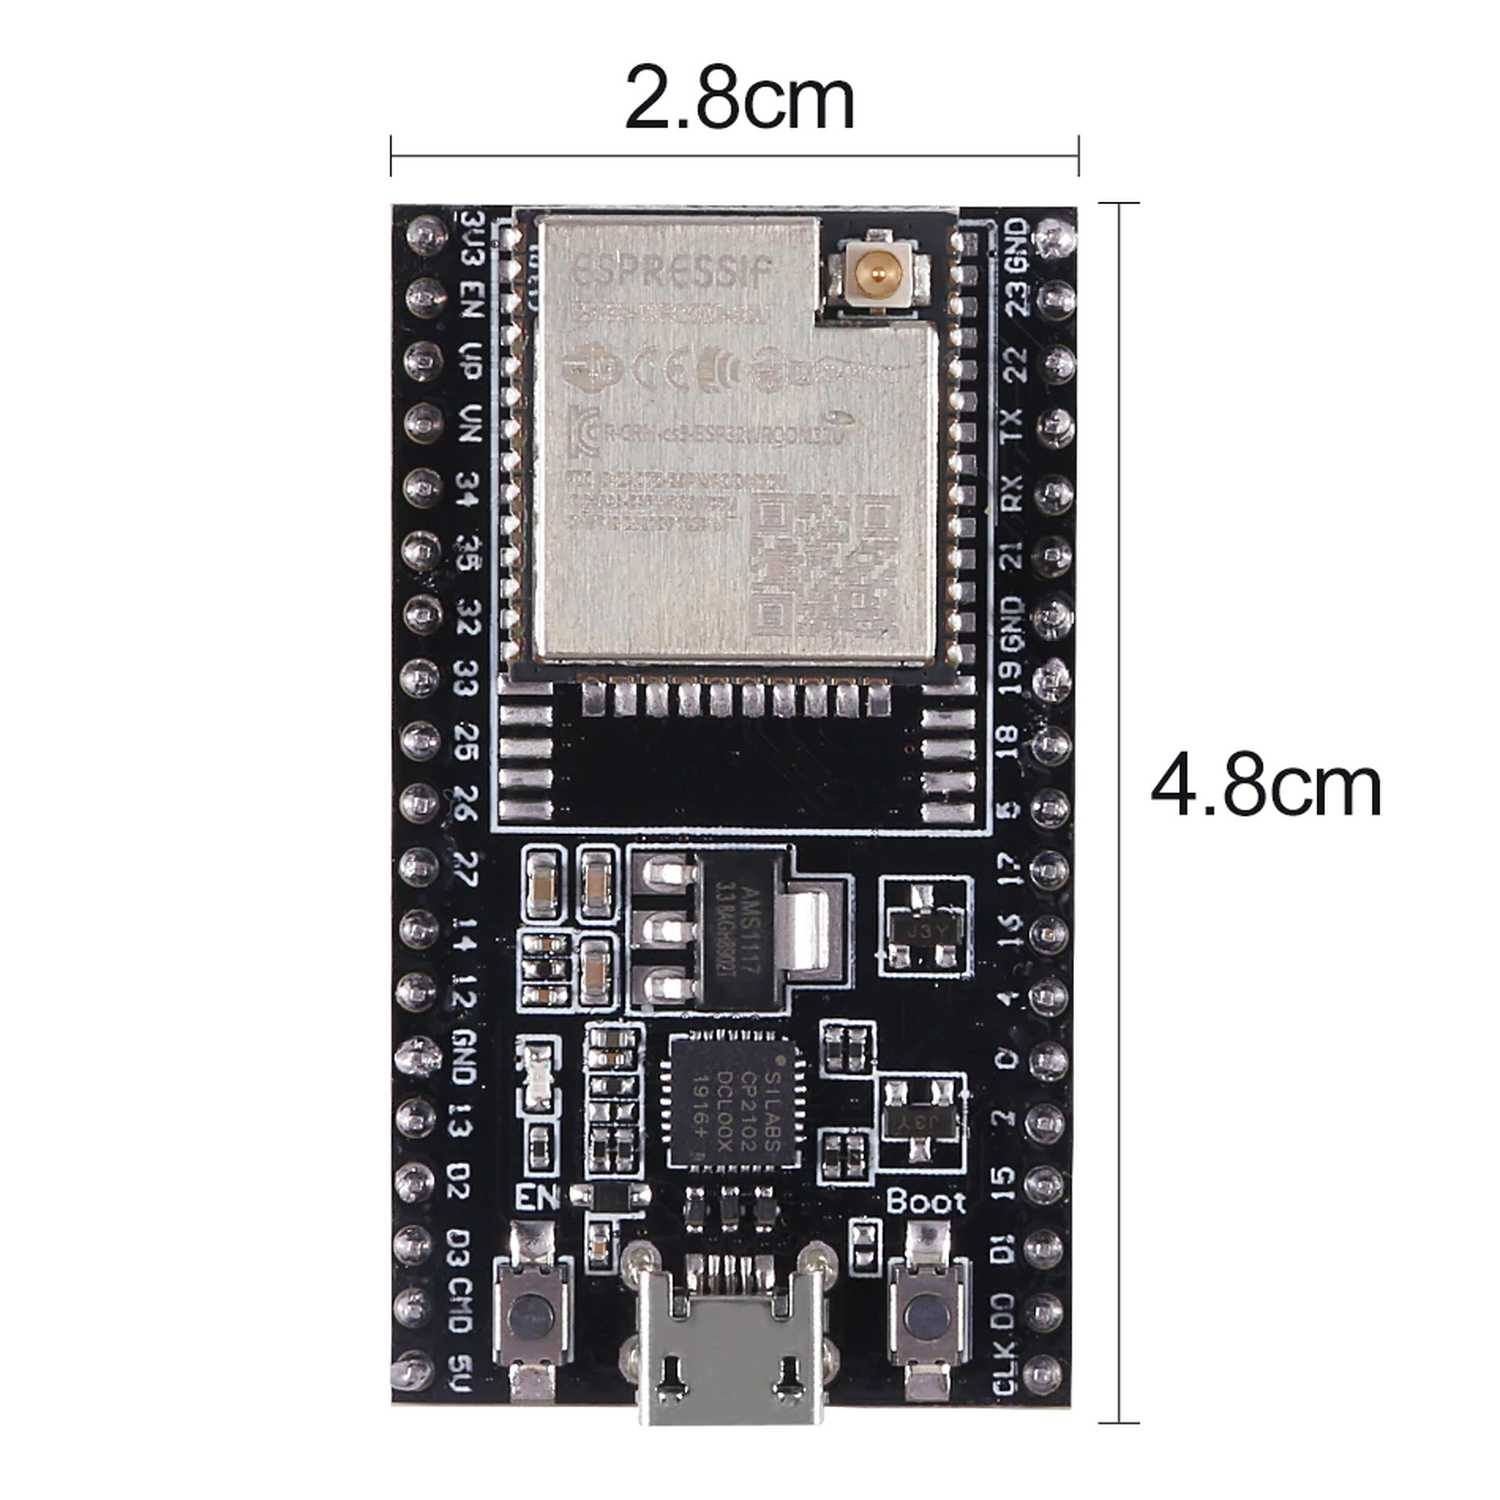
\includegraphics[width = 0.4\textwidth]{graphics/Produktbild_ESP32_2}
\caption{ESP32-32U DevKit.}
\label{fig:Produktbild_ESP32_32U_DevKit}
\end{figure}